\chapter{Human Pose Estimation (HPE)}
\vspace{-1cm}
\begin{figure}[h]
    \centering
    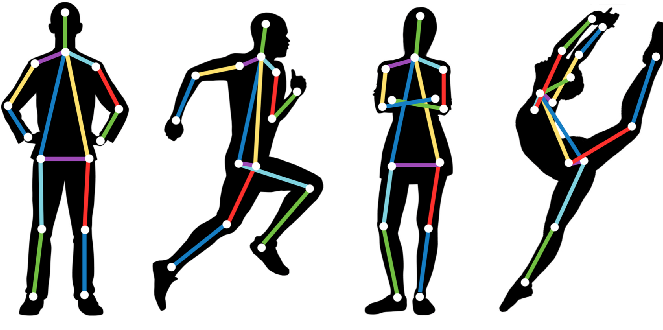
\includegraphics[scale=0.7]{img/hpe.png}
\end{figure}

\vspace{-0.5cm}
\section{Introduction, motivations and challenges}
\textbf{Human Pose Estimation (HPE)} deals with the estimation of the position of one or more human body within an image. HPE focuses on static body poses in individual frames, while HAR we have explained in the previous chapter looks at dynamic movement patterns across the video. How we will see at the end, human pose estimation can be used as input feature for HAR.
\vspace{-0.6cm}
\subsection{Applications of HPE}
The \textbf{applications} that HPE can find are: \textit{HCI} (Human-Computer Interaction), \textit{Virtual reality}, for realizing special effects in \textit{movies and animation}, sport motion analysis and also for video survelillance combined with HAR tasks.
\vspace{-0.5cm}
\subsection{Challenges related to Human Pose Estimation}
Like HAR, also HPE is a \textbf{very challenging computer vision task} for several reasons: (i) the human body is extremely flexible (high DOF), it suffer from self-occlusions (that is parts which are superimposed)...\\
\noindent
The \textbf{basic steps} are mainly: 
\begin{enumerate}
    \itemsep-0.3em
    \item Localizing human body (SPPE) or human bodies (MPPE) \textbf{joints/keypoints}; 
    \item Grouping them together into \textbf{valid configurations}.
\end{enumerate}

How you can imagine the problem of estimating the pose of multiple people within a scene is even more complicate. We will proceed step-by-step in the explanation analyzing the most popular models from simpler ones to achieve more complicate architectures.

\section{Single-Person Pose Estimation (SPPE)}

\subsection{DeepPose}
\textbf{DeepPose} is historically the first model which uses ConvNets for HPE. This model was introduced in \citedate{Toshev_2014} in the paper \citetitle{Toshev_2014}, \cite{Toshev_2014}. The problem of detecting the body joints is cast as a \textbf{DNN-based regression problem}, then the outputs are 2D body joint positions. A multi-stage architecture is implemented for prediction refinement and an \textit{holistic approach} is used in the sense that all joints are estimated even if not visible.

\subsubsection{DeepPose architecture}
\begin{figure}[h]
    \centering
    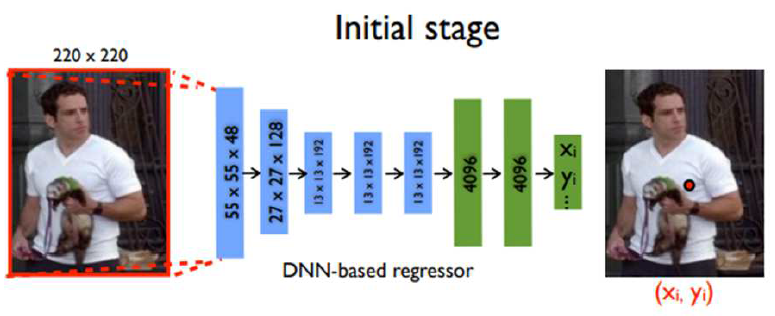
\includegraphics[scale=0.7]{img/DeepPose.png}
    \caption{DeepPose initial stage}
\end{figure}
The first step is an \textit{image preprocessing}, an object detector is used in order to find the person within the image; the original image, is then cropped taking as reference the bounding box information. As DNN backbone is used AlexNet, with an extra laye for predicting the (x,y) position of $k$ body joints. Since this is a regression task, a least-squares based loss can be used for training it. \\
After this initial stage, the estimated pose is passed through a cascade of three regressors in order to refine it by cropping the original image around the predicted point and passing it to the next-step regressor.
\vspace{-0.5cm}
\begin{figure}[h]
    \centering 
    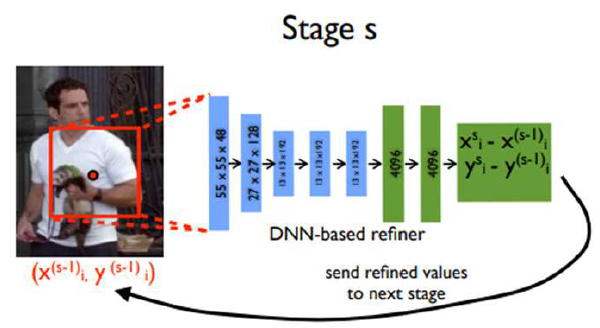
\includegraphics[scale=0.8]{img/DeepPose2.png}
    \caption{DeepPose: estimated pose refinement}
\end{figure}
DeepPose is the first CNN-based approach for estimating the pose of a single human body within a scene. The main limitation is that regressing joint positions is an extremely difficult task. More specifically, only regression is not sufficient to effectively solve the SPPE task. 


\subsection{ConvNet Pose: toward the use of heatmaps}
At this stage, after having introduced the first model, is shift the problem to the estimation of \textbf{heatmaps for joints} and then find coordinates as a second step according to the regions of major activation.
\begin{definition}[\textbf{Heatmap}]
    Given a joint, its heatmap is an \textit{image} where each pixel contains the probability that the joint is located there.
\end{definition}
\begin{figure}[h]
    \centering
    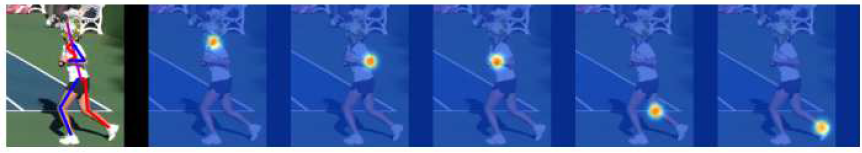
\includegraphics[scale=0.8]{img/HeatMap.png}
    \caption{Joints on a runner with related heatmaps}
\end{figure}

One of the first approaches for the computations of HeatMaps is presented in \citetitle{ConvNetPose} (\citeauthor{ConvNetPose}, \cite{ConvNetPose}) where a \textit{multiscale filtering approach} is used. The idea of refining predictions is kept from DeepPose and reused by following works on HPE.\\
\subsubsection{ConvNet Pose approach}
The model proposed in \cite{ConvNetPose}, follows a sliding-window approach, in particular it analyzes \textbf{three pyramidal versions} of the input and produces a \textit{coarse estimation} for both heatmaps and joint locations $(x,y)$. Such joint estimates are used to crop the features of the first conv layer which are fed into a module which refine the computed coarse heatmaps. This module outputs some heatmaps with $(\Delta{x}, \Delta{y})$ refinement these contribute to obtain the the final joint positions $(x,y)$. 

\begin{figure}[h]
    \centering
    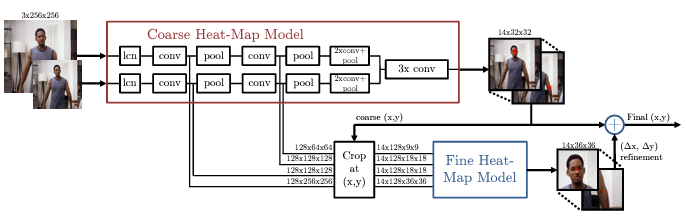
\includegraphics[scale=1]{img/ConvNetPose.png}
    \caption{Cascaded Architecture proposed in \cite{ConvNetPose}}
\end{figure}
The method lacks a structural model (either explicit or implicit) of the human joints that helps identify visible joints and only estimates occluded ones. For this model, the obtained results are far to be state of the art ones. The novelty in the next model we present is therefore the presence of an \textbf{implicit spatial model} for the human body.

\subsection{Convolutional pose machines (CPM)}
\textbf{Convolutional Pose Machines (CPMs)} proposed in \cite{wei2016convolutional} are based on the idea of \textit{pose machines}\footnote{Which in turn use \textit{inference model} to carry out the job } which is a sequence of predictors trained to \underline{identify joint locations}. The approach combines information of multiple joints to solve the ambiguities, in this way an implicit spatial model of the human body is used. 

\begin{figure}[h]
    \centering
    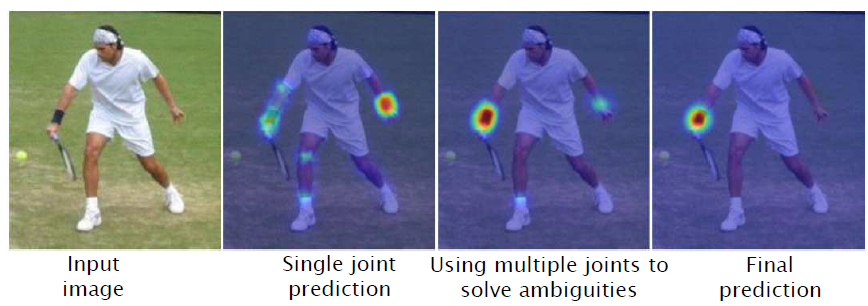
\includegraphics[scale=0.7]{img/CPM1.png}
    \caption{Solving the ambiguities using multiple joint heatmaps}
\end{figure}
The image above shows the predictions for the left wrist in which there is an ambiguity with the right one, using the heatmap of the right wrist, such an ambiguity can be solved generating a correct final prediction. This implicitly provides the model with a description of what is the left wrist and what the right wrist.

\subsubsection{CPM architecture}
A CPM consists of two or more stage, where each stage contains a \textbf{multi-class heatmap predictor} $g$, it is an architecture which is trainable end-to-end (since the whole structure is differentiable and the backpropagation can be correctly performed).\\
The \textbf{first stage} computes initial predictions for joint locations; the \textbf{following stages} takes as input the image features (again) and the heatmaps computed at previous stage these acts as \textbf{context features}. Context features help eliminate wrong estimations while strenghtening correct ones on a single heatmap. It is remarkable that each stage is supervised independently during the training using the ground truth heatmap.

\begin{figure}[h]
    \centering
    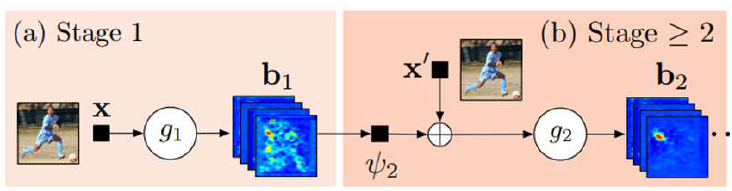
\includegraphics[scale=1]{img/CMP_arch.png}
    \caption{Convolutional Pose Machine architecture}
\end{figure}

We have introduced in the chapter about Object Detection, the concept of \textit{receptive field}. Well, here this plays  a crucial role, since the use of a larger receptive fields across different layer helps to capture \textbf{long-range \underline{spatial} dependencies}. In the following the effect of refining the heatmaps is shown.

\begin{figure}[h]
    \centering
    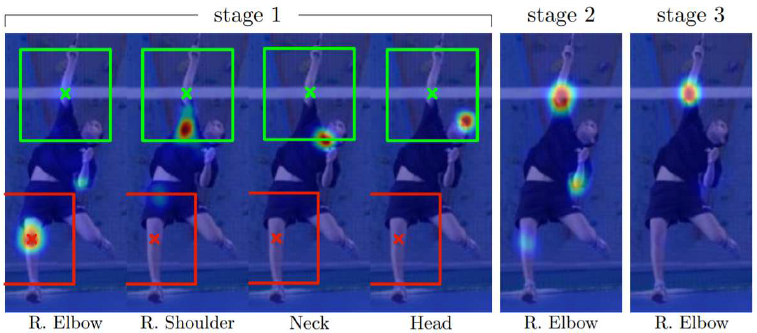
\includegraphics[scale=0.8]{img/CPM_2.png}
    \caption{\textbf{Effect of heatmaps refinement} The estimated heatmap for the Right elbow is completely wrong in the first stage, in the second stage using context features there is an improvement, in the third stage the heatmap is completely correct}    
\end{figure}


\section{Multiple-Person Pose Estimation(MPPE)}
\vspace{-0.6cm}
\begin{figure}[h]
    \centering
    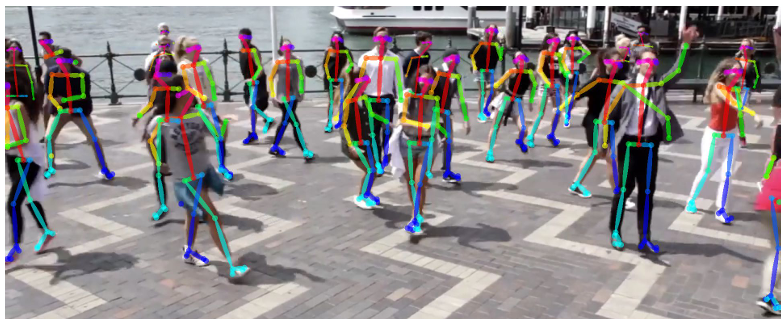
\includegraphics[scale=1]{img/OpenPose6.png}
\end{figure}
\noindent
When the task is \textbf{estimating the pose of multiple person} (MPPE) there are even more difficulties since both position an number of hummans in a certain image is unknown. There are tipically two ways to implement MPPE: 
\begin{itemize}
    \itemsep-0.3em
    \item \textsf{Top-down approaches} In this case, first a person detector outputs a list of candidate bounding boxes that are further analyzed to extract the pose for each person. This apparently seems simpler because you can iteratively apply (for each person) a CPM (for example). However, this is strongly dependent on the accuracy of the person detector, and the execution time, clearly, is proportional to the number of people of which estimate the pose;
    \item \textsf{Bottom-up approaches} First detect \textbf{all the possible joints} (for each person), and then try to associate joints belonging to the same person. This is a very difficult task in a complex environment.
\end{itemize}  

\subsection{OpenPose: real-time MP 2D Pose Estimation using PAFs}
\textbf{OpenPose} (see \cite{openpose}) can be seen as an extension of CPM, since a multi-branch architecture is considered. It combines the \textbf{extraction of heatmaps} with thatof a non-parametric representation (Part Affinity Fields) aimed at learning to associate body parts with different individuals. So, one branch is for the heatmaps (like in CPM), the other is related to the PAFs computation.  Both \textit{heatmaps} and \textit{PAFs} are refined step-by-step.

\subsection{The OpenPose method}
The steps by which OpenPose solves the MPPE problem is the following. During the explanation some topics (eg. PAF) will be better formalized: 

\subsubsection{1. Extract frame features}
The frame features $\mathbf{F}$ are computed using a fine-tuned VGG-19 architecture as feature extractor. Such architectures used in principle for image classification are very good tools for deriving the useful features from the frame to be analyzed.
\subsubsection{2. Heatmaps and PAFs}
From features \textbf{F}, both \textbf{heatmaps} $\mathbf{S}^t$ (in the paper are called \textit{saliency maps}) and \textbf{Part Affinity fields} $\mathbf{L}^t$ are estimated. One heatmap per joint ($J$ joints in total) and one PAF per limb\footnote{
    Note that a limb is related to a couple of keypoints.
} (C limbs in total) are computed. Here $t\ge{1}$ indicate the $t$-th stage. 

\begin{figure}[h]
    \centering
    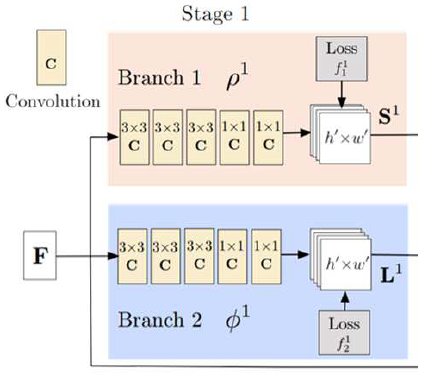
\includegraphics[scale=1]{img/OpenPose1.png}
    \caption{The two branch of OpenPose architecture}
\end{figure}

\subsubsection*{\textsf{Part Affinity fields}}
A \textbf{Part Affinity Field (PAF)} encodes a spatial non-parametric relationship between different body parts. For each limb, a PAF represents association scores between joints as a set of \textbf{2D vector fields}. These vector fields encode: (i) the location and orientation of limbs in the image; (ii) the relationship between pairs of keypoints (eg. shoulder-elbow, wrist-hand...). The important thing to remind is that PAFs help in identifying which body parts belong to the same individual MPPE.

\begin{figure}[h]
    \centering
    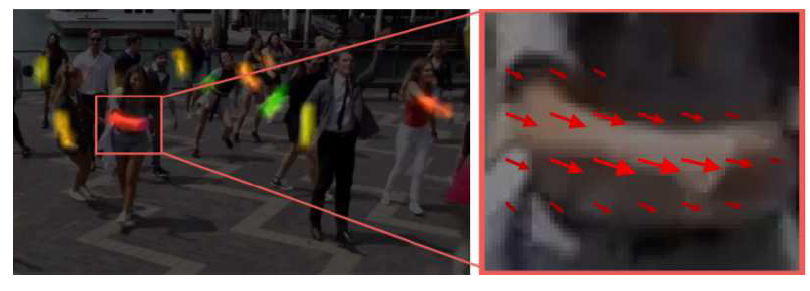
\includegraphics[scale=0.8]{img/PAF.png}
    \caption{Part Affinity fields in a frame with multiple people}
\end{figure}

\subsubsection{3. Refining detections and associations}
From stage 2 onwards, detections (heatmap) and association (PAFs) are refined simultaneously exploting information from the previous stage
    $\{\mathbf{F},\ \mathbf{S}^{t-1}, \ \mathbf{L}^{t-1} \}$
In particular we have that: 
\begin{align}
    &\mathbf{S}^t = \rho^t(\mathbf{F},\mathbf{S}^{t-1}, \mathbf{L}^{t-1}), \quad \forall{t}\ge{2}\\
    &\mathbf{L}^t = \phi^t(\mathbf{F},\mathbf{S}^{t-1}, \mathbf{L}^{t-1}), \quad \forall{t}\ge{2}
\end{align}

\begin{figure}[h]
    \centering
    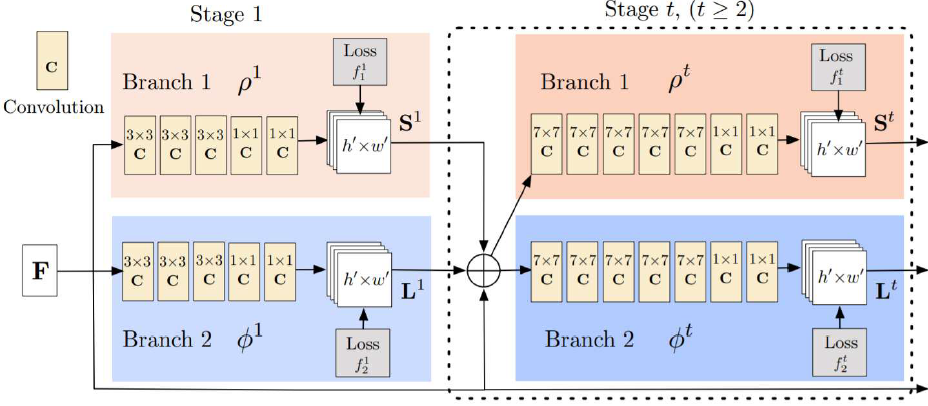
\includegraphics[scale=0.7]{img/OpenPose2.png}
    \caption{Complete OpenPose architecture with $t\ge{2}$}
\end{figure}
where $\rho$ and $\phi$ are the transformations coming from the convolutional layer, respectively, in the Branch 1 and Branch 2.

\subsubsection{4. Part association}
Once we have joint positions and PAFs, we have to associate parts to people. It was not a case the fact we add an additional branch to the architecture, indeed using only joint positions/heatmap leads to false association between limbs and individuals. On the other hand, if you combine joint information and PAFs, structural information can be provided.

\begin{figure}[h]
    \centering
    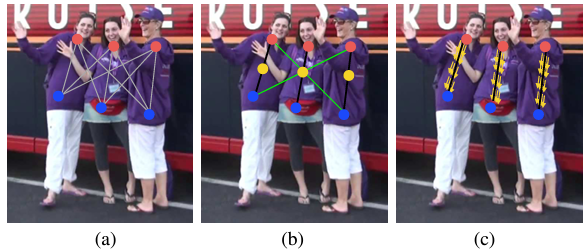
\includegraphics[scale=0.9]{img/OpenPose3.png}
    \caption{Part association strategies. (a) The body part detection candidates (red and blue dots) for two body part types and all connection candidates (grey lines). (b) The connection results using the midpoint (yellow dots) representation: correct connections (black lines) and incorrect connections (green lines) that also satisfy the incidence constraint. (c) The results using PAFs (yellow arrows). By encoding position and orientation over the support of the limb, PAFs eliminate false associations.}    
\end{figure}

\subsubsection*{Assignment algorithm}
Given the \textbf{complete bipartite graph of possible connections}, assign a weight to each edge as the \textit{line integral} along the segments in the corresponding PAF for that limb. At this point we have to find connections that maximize the total weight. There are many solutions to solve this problem, for example: (i) sort the connections by weight; (ii) pick iteratively the highest weight corresponding to a connection whose endpoints have not been already chosen. At the end of this procedure we have a list of keypoints which are owned by the same person.

\begin{figure}[h]
    \centering
    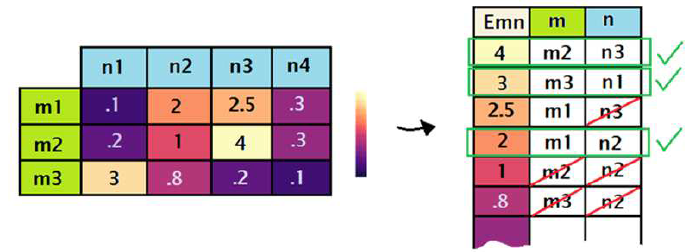
\includegraphics[scale=0.8]{img/OpenPose4.png}
    \caption{Assignment algorithm}
\end{figure}


\subsubsection{5. Merging}
The last step is iteratively merging parts. A greedy approach is used where, at first each part is associated to an individual, if two individuals share an endpoint, they are the same human, we merge the keypoints in the same set, we remove a human. This procedure is repeated until the list is not empty.

\begin{figure}[h]
    \centering
    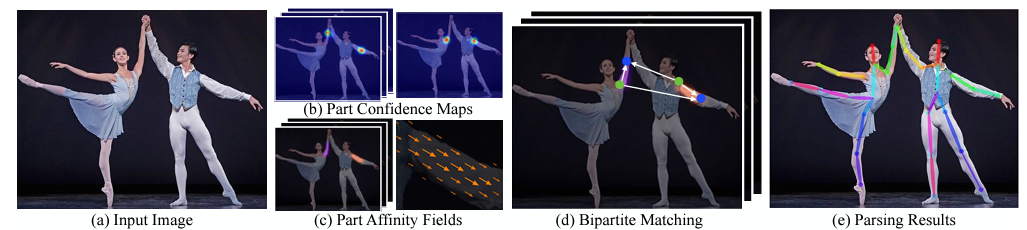
\includegraphics[scale=0.8]{img/OpenPose5.png}
    \caption{\textbf{OpenPose overall pipeline}. (a) Our method takes the entire image as the input for a CNN to jointly predict (b) confidence maps for body part detection and (c) PAFs for part association. (d) The parsing step performs a set of bipartite matchings to associate body part candidates. (e) We finally assemble them into full body poses for all people in the image.}
\end{figure}

\newpage
\subsection{The state-of-the-art model: DeepCut}
In the \citedate{DeepCut}, \citeauthor{DeepCut} (see \cite{DeepCut}) introduced a bottom-up approach, called \textbf{DeepCut} which jointly solves the task of detecting and estimating the pose of multiple person. The approach is not so easy, since involve the formulation and the solution of an NP-Hard optimization problem. We will give only the main steps and ideas, a more detailed description of all the points treated here can be found in the original paper \cite{DeepCut}.\\
 The approach combines a set of \textbf{joint hypotesis} (computed with a CNN detector (Faster RCNN)) with an instance of a particular  optimization problem called the \textbf{ILP} (Integer Linear Program) which implicitly perform a sort of NMS\footnote{Non-max suppression} of the candidate parts and groups them to form \textbf{configurations of body parts} respecting \underline{constraints} of geometry and appearance. The main steps are the following: 
\begin{enumerate}
    \itemsep-0.3em
    \item A subset of joints from an initial set of D candidates is selected (these ore obtained by a detector + class probabilities); 
    \item We label each selected candidate as an individual joint ($C$ total classes); 
    \item Partition body parts that belongs to the same person and retrieve valid pose configurations.
\end{enumerate}
State-of-the-art results have been obtained for both MPPE and SPPE problem. For the sake of clarity, we take the image from the paper \cite{DeepCut} with the associated caption. 

\begin{figure}[h]
    \centering
    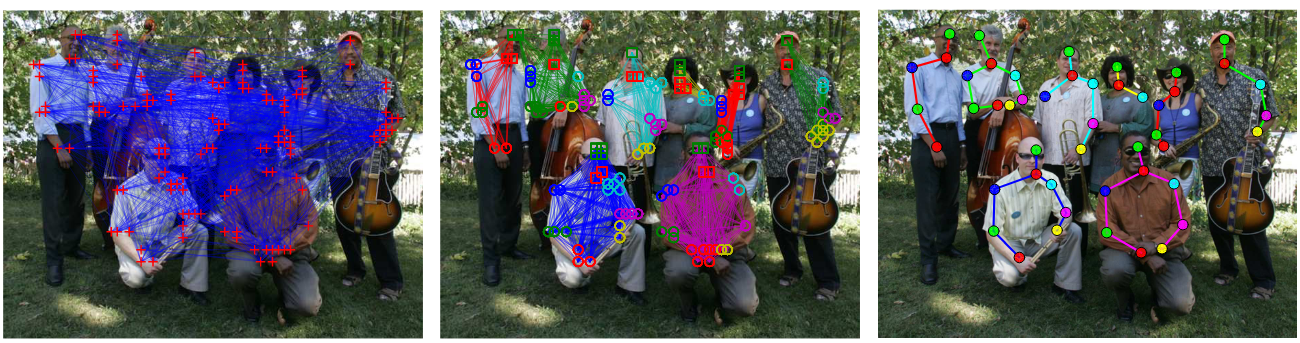
\includegraphics[scale=0.6]{img/DeepCut1.png}
    \caption{\textbf{DeepCut method overview}. (a) initial detections (= part candidates) and pairwise terms (graph) between all detections that (b) are jointly clustered belonging to one person (one colored subgraph = one person) and each part is labeled corresponding to its part class (different colors and symbols correspond to different body parts); (c) shows the predicted pose sticks.}
\end{figure}

\subsubsection{The core of DeepCut: ILP (Integer Linear Program)}
The \textbf{Integer Linear Program (ILP)} is the core of the method. It deals with the previous three steps as triple of binary variables $(x,y,z)$. Where, in particular:
\begin{itemize}
    \itemsep-0.2em
    \item $x(d,c)=1$ if the joint candidate $d\in{D}$ belongs to joint class $c\in{C}$; 
    \item $y(d,d')=1$ if candidates $d$ and $d'$ belongs to the same person; (inter-person)
    \item The variable $z$ is used to \textbf{partition pose} belonging to different people; in particular $z(d,d',c,c')=x(d,c)\cdot{x(d',c)}\cdot{y(d,d')}=1$ if $d$ and $d'$ are of class $c$ \underline{and} belongs to the same person.  (intra-person)
\end{itemize}

\subsubsection*{\textsf{Constraints of ILP}}
The \textbf{constraints} of ILP are the  following:
\begin{itemize}
    \itemsep-0.3em
    \item \textbf{Uniqueness} each joint $d$ must belong to only one class $c$
    \begin{equation*}
        \forall{d}\in{D}: \quad \sum_{c\in{C}} {x_{dc}}\le{1}
    \end{equation*}
    \item \textbf{Consistency} two different body parts  $d$ and $d'$ belongs to the same person if and only if neither $d$ or $d'$ have been suppressed.
    \begin{align*}
        &\forall{dd'}\in\binom{D}{2}: \ y_{dd'} \le \sum_{c\in{C}} x_{dc}\\
        &\forall{dd'}\in\binom{D}{2}: \ y_{dd'} \le \sum_{c\in{C}} x_{d'c}
    \end{align*}
    \item \textbf{Transitivity} for any triple of candidate parts $d$, $d'$, $d''$ if $d,d'$ are of the same individual and the same holds for $d',d''$ then also $d,d''$ belongs to the same person.
    \begin{equation*}
        \forall{dd'd''}\in\binom{D}{3}: \ y_{dd'}+y_{d'd''}-1\le{y_{dd''}}
    \end{equation*}
\end{itemize}
The set of all feasible solutions (the solutions which satisfy the constraints) with the notation $X_{DC}$. Once we have defined it, we can give the complete optimization problem formulation. 


\subsubsection*{\textsf{Objective function of ILP}}
The objective functions is composed of a sum of two terms one accounting for the \textbf{part labeling} and the \textbf{part clustering}: 
\begin{equation}\label{eq:ILP}
    \min_{(x,y)\in{X_{DC}}} {
        \sum_{d\in{D}}\sum_{c\in{C}} \alpha_{dc}x_{dc} 
    }+
    {
        \sum_{dd\in\binom{D}{2}} \sum_{c,c'\in{C}} \beta_{dd'cc'} x_{dc}x_{d'c}y_{dd'}
    }
\end{equation}
Just to mention, such problem is solved by using a branch-and-cut approach using the state-of-the-art ILP solver Gurobi. More specifically a sequence of relaxed version of the problem \ref{eq:ILP} is computed, until a satisfactory optimality gap is achieved.

\subsubsection*{\textsf{Pose sticks prediction}}
After solving the ILP, the selected keypoints are connected based on the \textbf{predefined skeleton structure}, creating the "pose sticks" which are drawn directly using on the image using the reference model itself.
 
\subsection{AlphaPose: Regional Multi-Person Pose Estimation (RMPE)}
This is a top-down approach and it is based on the observation that the pose estimator module suffer from inaccurate predictions of the person detector module. For this reason, first is applied a single-person pose extractor (SPPE), which for sure will result in redundant and inaccurate poses, then the RMPE is applied to eliminate the previous issues. \\
The main advantage is that is a very general framework in which any person dector and single pose estimators can be used.

\subsubsection{AlphaPose architecture}
\begin{figure}[h]
    \centering
    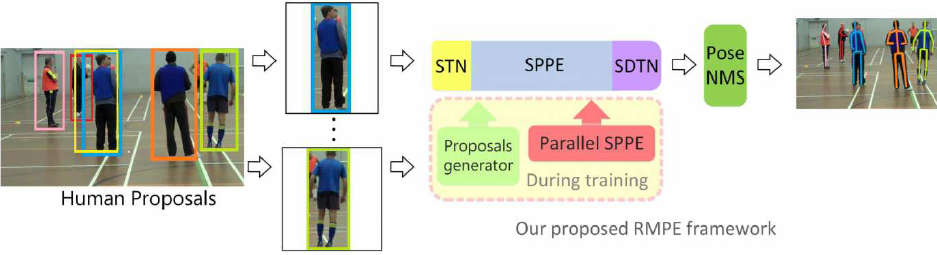
\includegraphics[scale=0.9]{img/AlphaPoseArch.png}
    \caption{AlphaPose architecture}
\end{figure}

\noindent
Human bounding boxes coming from the human detector (whatever you want to use) are fed to a sequence of modules which compose a \textbf{human pose proposal generator} (STN+SPPE+STDN), which generates pose estimates. Pose estimates are then refined by using a Non-max suppression module (NMS). Let us a slightly more detailed description of the human pose proposals module: 
\begin{itemize}
    \itemsep-0.3em
    \item The \textbf{Spatial transformer Network} (STN) selects and centers the \textit{dominant region} in which there is the human 
    \item ...in order to simplify the work to the Single Person Pose Estimator (SPPE); 
    \item After that, a de-transformer module called \textbf{Spatial De-transformer Network}(SDTN) remaps the original coordinates. 
    \item \textit{During the training} a parallerl SPPE branch works as a regularizer that penalizes poses which are not well-centered.
    \item After having proposed the poses, the \textbf{NMS} module comes into play. This is a \textit{trainable module} whose objective is eliminate redundancies by using some \textit{elimination criterion (EC)}\footnote{
        This is usually based on pose similarity and pose distances: two poses which are very close each other probably are redundant and \textbf{the most confident one} must be selected.
    }
\end{itemize}

\section{The Coco Keypoints structure}
We have understood that, at the end of the day we want to superimpose pose sticks on images according to a certain \textbf{scheleton structure}. Among all the possible reference model, we cite an example for the \textbf{COCO dataset}, in which 18 keypoints are used in order to describe the poses.

\begin{figure}[h]
    \centering
    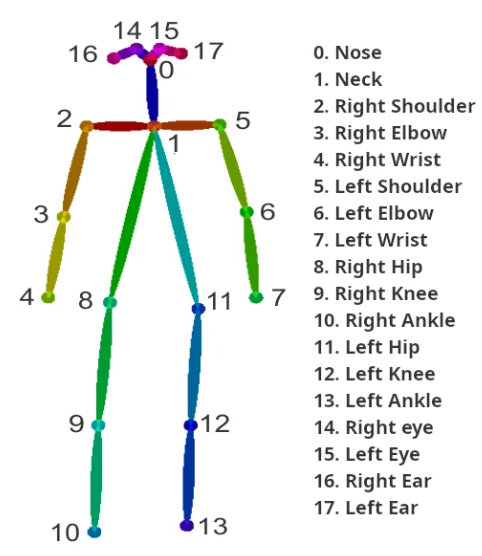
\includegraphics[scale=0.8]{img/Coco_Poses.png}    
    \caption{Skeleton structure and Keypoints description}
\end{figure}

\section{Conclusion}
Different models for single and multiple human pose estimation have been proposed. Moreover, different top-down and bottom-up approaches have been introduced, highlighting what are main features, advantages and disadvantages of each one.\\
HPE feature can guide the complex Human Action Recognition (HAR) task: certain poses can lead to the exclusion of some actions with respect to the other. As an advice, a complete explanation for the proposed models can be found by following the references to the bibliography at the end of these lecture notes book.



